\chapter{New Ultrashort X-ray Sources}\label{Ultrashort X-ray Sources}\noindent
 
Since the discovery of X-rays by Wilhelm R\"{o}ntgen in 1895 X-ray sources have
continuously improved, often leading to significant new science. The increase in
brilliance since the first rotating anodes used for crystallography has been
spectacular, bridging many orders of magnitude. The development of second
generation light sources in the beggining of the 80s dedicated exclusively to
the production of synchrotron light contributed to an explosion of
protein structures solved by crystallography which continued to accelerate with
the introduction of widdlers undulators and the increase in brightness from
third generation sources.

 
\begin{figure}[h]
\centering
  \includegraphics[width=1.0 \columnwidth]{brilliance.pdf}
  \caption{Peak brilliance of several X-ray sources.}
%    http://www.nature.com/nphoton/journal/v1/n6/abs/nphoton.2007.76.html and TESLA_Technical_design_Report
  \label{Fig:Brilliance}
\end{figure}

The introduction of free electron lasers brings with it an increase in peak
brightness comparable to the change from rotating anodes to synchrotron sources
(Fig. \ref{Fig:Brilliance}). They also offer very high coherence and ultra fast
pulses of only a couple of femtoseconds opening a new window into the world of
ultra fast science. HHG sources also shares many of the characteristics of free
FELs albeit with lower peak power. In this chapter we will try to provide an
overview of these two light sources.

\section{Free electron lasers}

Free electron lasers are in many ways an evolution from third generation
synchrotrons and so they are often called fourth generation light sources. The
fundamental difference between these two light sources is that while in a
synchrotron photons are generated independently of each other in a free electron
laser photon are generated in phase with each other and so cooperate to produce
a pulse which has an intensity proportional to the square of the number of
electrons being accelerated, instead of being linear with the number of
electrons as is the case for a synchrotron.

\subsection{The SASE process}

The SASE process, central to all existing X-ray free electron lasers, is a
process in which the electrons are organized in micro bunches separated by the
distance of a wavelength, as they go through the undulator (see
Fig. \ref{Fig:Brilliance}). This happens because,
as in a normal synchrotron, when the electrons go through the undulator they
will emit radiation due to the acceleration of imposed by the magnetic field. If
the undulator is sufficiently long this radiation will starts to produce a
measurable effect in the distribution of the electrons making them accumulate in
micro bunches separated by exactly one wavelength. This is a self reinforcing
process as the more the electrons bunch together the stronger the field they
produce as they will radiate coherently. This process continues until almost all
the electrons are in these micro-bunches, at which point it is said that
saturation is reached. 

\begin{figure}[h]
\centering
  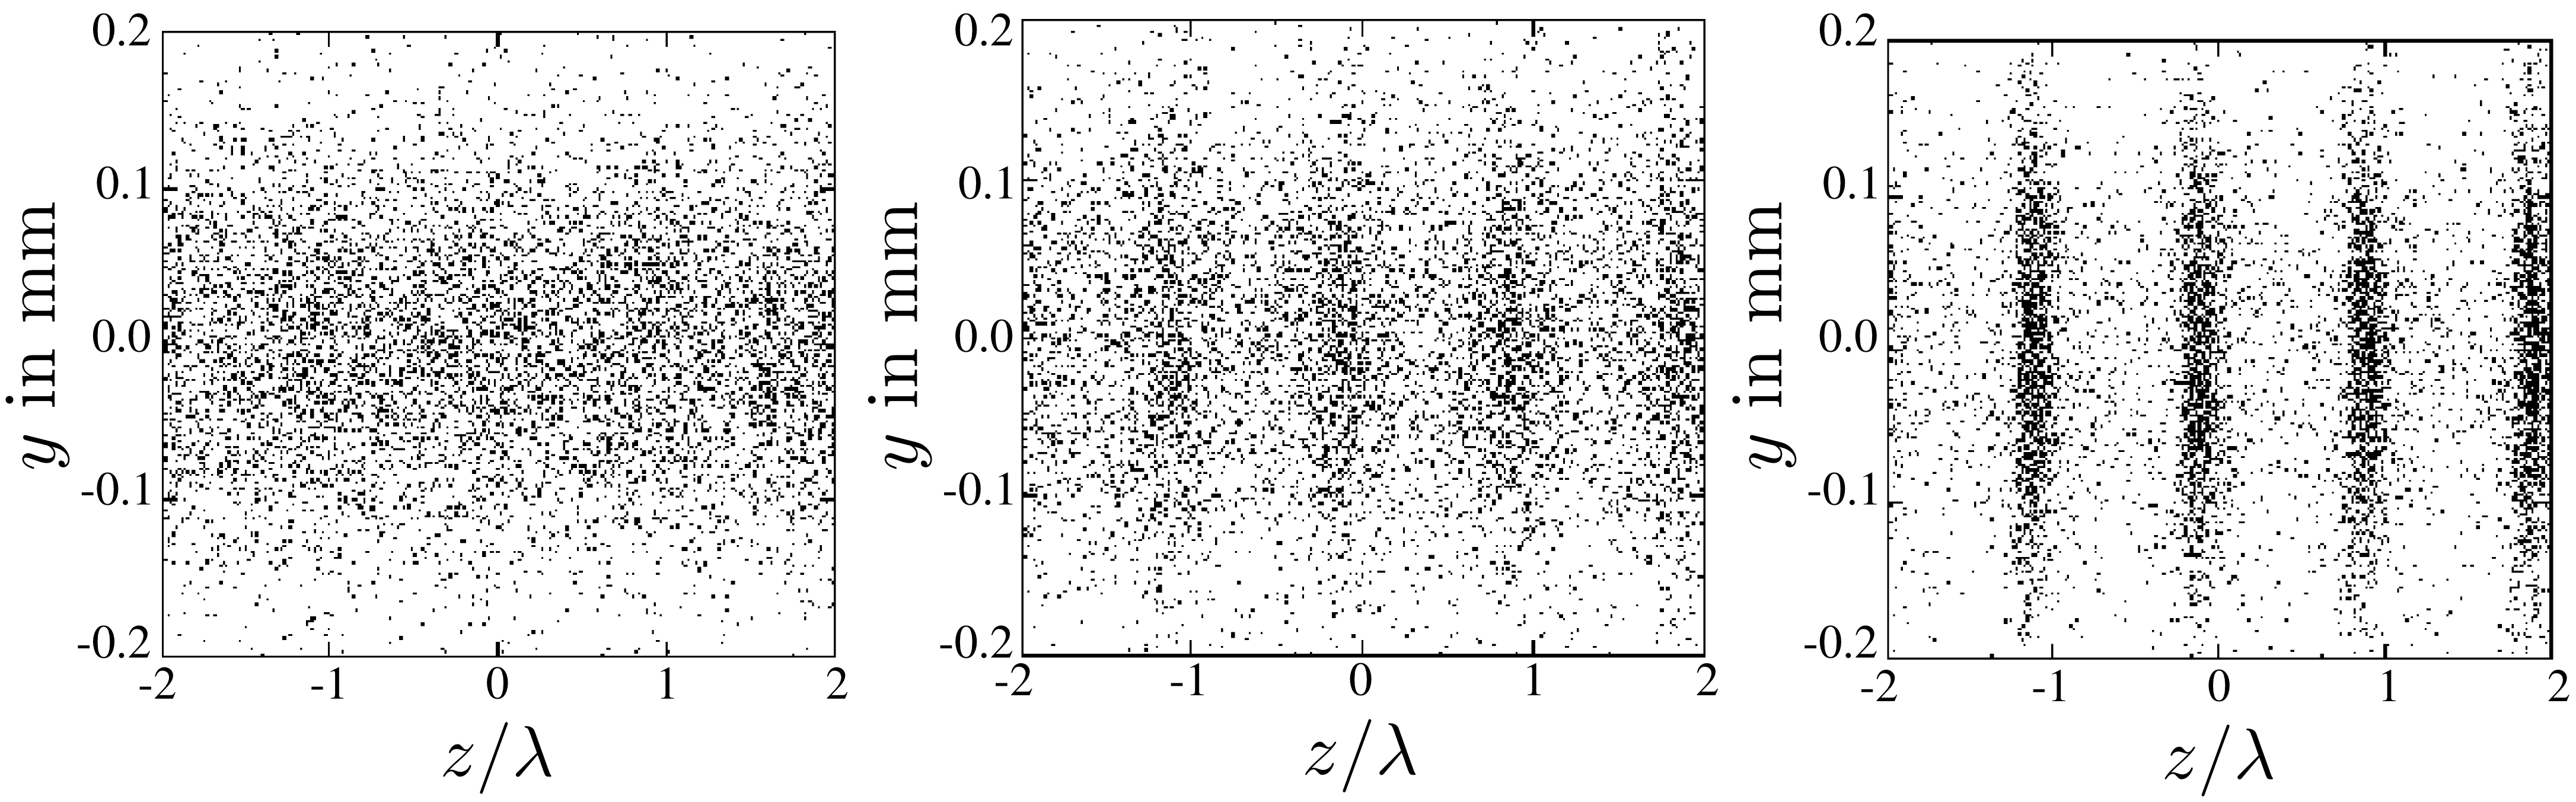
\includegraphics[width=1.0 \columnwidth]{micro-bunching.png}
  \caption{Simulation of micro-bunching during the SASE process where the
    electron density is represented by the density of dots. The snapshots
    from the left to the right represent the electron structure along the
    undulator, with the left side representing the beggining and the right side
    the end of the undulator. \ref{TESLA_Technical_design_Report}}
  \label{Fig:Brilliance}
\end{figure}

The radiation produced by electrons distributed in this manner is much more
intense than if the electrons were uniformly distributed throughout the
undulator because with microbunching the distance between most of the electrons is
always a multiple of the wavelength, and so the radiated electric fields will be
in phase. In other words the electrons radiate coherently and the resulting
intensity will scale will the square of the number of electrons which is why the
difference in peak brilliance is so large.

\subsection{Current X-ray FEL Facilities}

X-ray FEL are developing at a very fast pace. E
Nowadays there is only one hard X-ray FEL facility, LCLS at SLAC, USA and one
one soft X-ray FEL named FLASH in DESY, Germany. But there are several X-ray FEL
being built such as the european XFEL in Germany and SCSS
in Japan both hard X-ray FEL as well as several soft X-ray sources such as FERMI
in Italy. The SwissFEL in Switzerland is also in planning stages. 
Due to the fact that X-ray FEL use linear accelerators it is only
possible to have beam in one beamline at the same time so even though the number
of facilities is increasing quickly, access to an X-ray FEL will continue to be
severely limited. This in combination with the different characteristics of FEL
radiation compared to a third generation synchrotron mean that while they are
often called fourth generation sources they will not replace synchrotrons in any
meaninful sense as it happened in the past. They should be considered a class of
their own better suited for other kinds of experiments not possible at synchrotrons.

\section{High harmonic generation}

The first High harmonic generation (HHG) sources were discovered about two decades ago
and since then their power has been increasing as the power of optical lasers
increases. They provide a relatively cheap source and tunable source of very
short (a few fs) and intense pulses (more than $10^{10}$ photons per pulse). 

HHG works by shining a very intense optical laser in a gas. When the field of
the optical laser is sufficiently strong the electron in the gas will be ionized
by field ionization, and as the field progresses they will be accelerated back
towards the ion and finally recombine, generating in the process short
wavelength radiation (see Fig. \ref{Fig:HHG_Process}).

\begin{figure}[h]
\centering
  \includegraphics[width=1.0 \columnwidth]{hhg-process.png}
  \caption{Simulation of micro-bunching during the SASE process where the
    electron density is represented by the density of dots. The snapshots
    from the left to the right represent the electron structure along the
    undulator, with the left side representing the beggining and the right side
    the end of the undulator. \ref{TESLA_Technical_design_Report}}
  \label{Fig:HHG_Process}
\end{figure}

* High Harmonic Generation

- Started one decade ago
- Short description with non linear effects
- Show some scheme of the setup
- Very short pulse lengths
- 
%%% Local Variables: 
%%% mode: latex
%%% TeX-master: "Thesis"
%%% End: 
